
\begin{frame}{B/P-spline base learner}
  \vspace{-0.3cm}\[g_k(x) = (B_{k,1}(x), \dots, B_{k,d_k}(x))^\tran\] B-spline basis $B$ of a pre-defined degree~\citep{eilers1996flexible}.
  \begin{center}
    \begin{figure}
      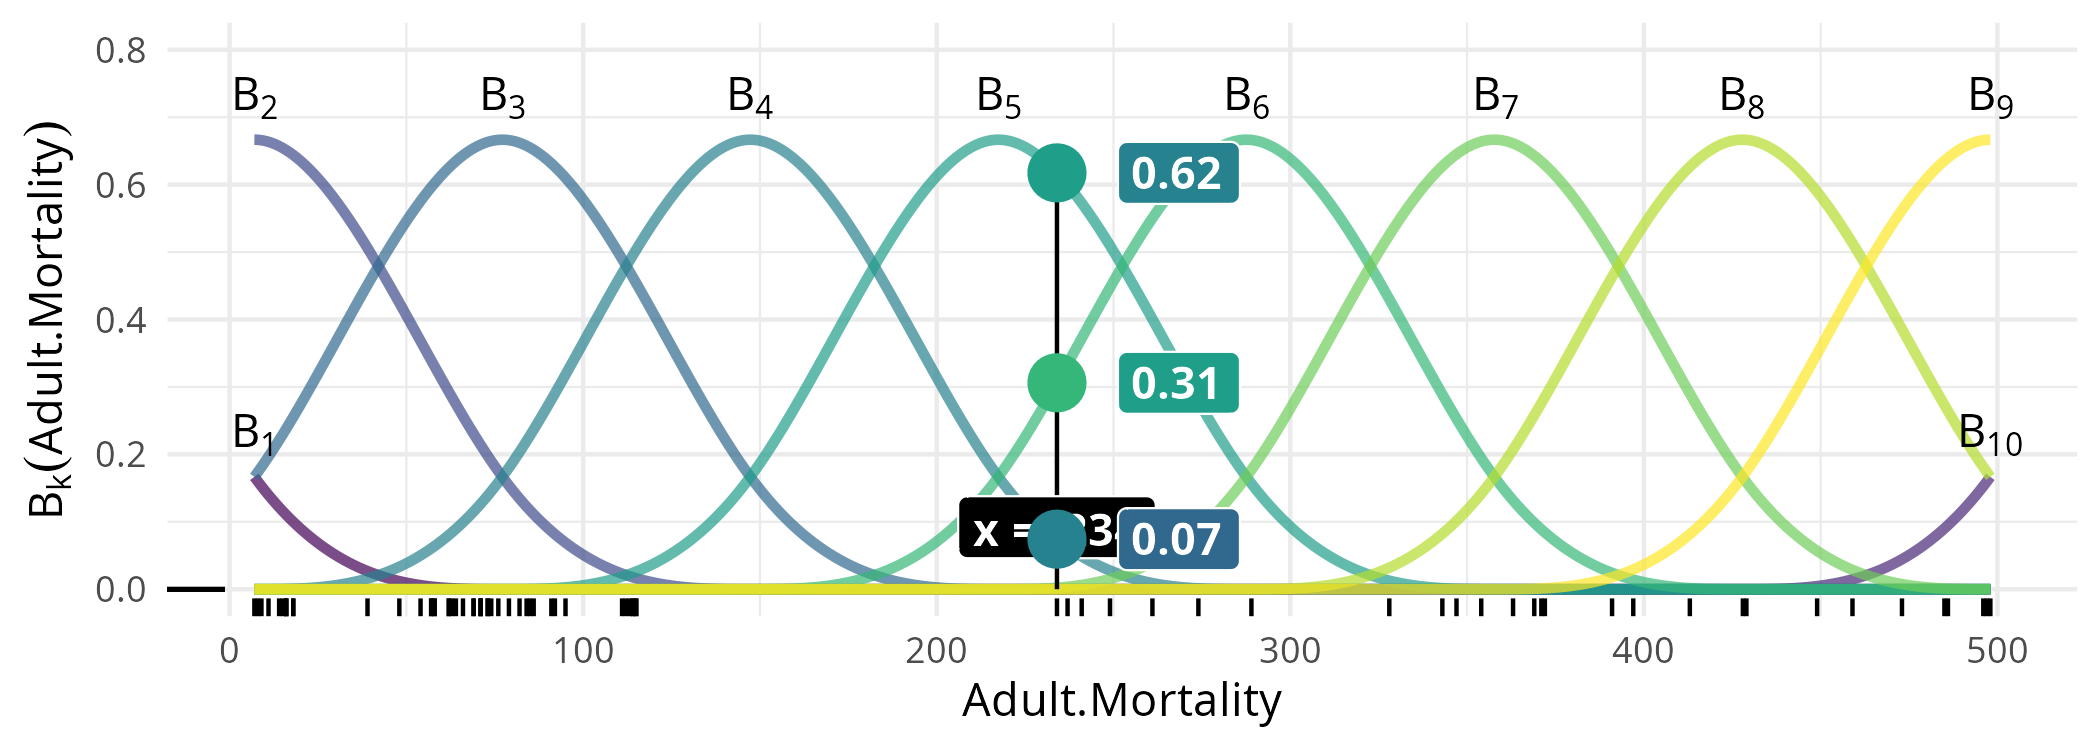
\includegraphics[width=0.7\textwidth]{figures/bs-base/fig-bs1.png}
    \end{figure}
  \end{center}
  
\[
\design_k = \tiny\begin{blockarray}{cccccccccc}
\color[HTML]{440154}B_{1} & \color[HTML]{482878}B_{2} & \color[HTML]{3E4A89}B_{3} & \color[HTML]{31688E}B_{4} & \color[HTML]{26828E}B_{5} & \color[HTML]{1F9E89}B_{6} & \color[HTML]{35B779}B_{7} & \color[HTML]{6DCD59}B_{8} & \color[HTML]{B4DE2C}B_{9} & \color[HTML]{FDE725}B_{10} \\
\begin{block}{(cccccccccc)}
\phantom{x}\\
\color{lightgray}0.00 & \color{lightgray}0.00 & \color{lightgray}0.00 & \color[HTML]{31688E}0.07 & \color[HTML]{26828E}0.62 & \color[HTML]{1F9E89}0.31 & \color{lightgray}0.00 & \color{lightgray}0.00 & \color{lightgray}0.00 & \color{lightgray}0.00\color{black}\\
\end{block}
\color{white}0.00 & \color{white}0.20 & \color{white}0.66 & \color{white}0.14 & \color{white}0.00 & \color{white}0.00 & \color{white}0.00 & \color{white}0.00 & \color{white}0.00 & \color{white}0.00\color{black}\\
  \color{white}0.00 & \color{white}0.00 & \color{white}0.00 & \color{white}0.00 & \color{white}0.00 & \color{white}0.00 & \color{white}0.00 & \color{white}0.17 & \color{white}0.67 & \color{white}0.17\color{black}\\
  \color{white}\vdots & \color{white}\vdots & \color{white}\vdots & \color{white}\vdots & \color{white}\vdots & \color{white}\vdots & \color{white}\vdots & \color{white}\vdots & \color{white}\vdots & \color{white}\vdots\\
  \color{white}0.00 & \color{white}0.02 & \color{white}0.48 & \color{white}0.48 & \color{white}0.02 & \color{white}0.00 & \color{white}0.00 & \color{white}0.00 & \color{white}0.00 & \color{white}0.00\color{black}\\
  \color{white}0.00 & \color{white}0.00 & \color{white}0.00 & \color{white}0.01 & \color{white}0.40 & \color{white}0.55 & \color{white}0.04 & \color{white}0.00 & \color{white}0.00 & \color{white}0.00\color{black}\\
  \color{white}0.00 & \color{white}0.00 & \color{white}0.00 & \color{white}0.00 & \color{white}0.00 & \color{white}0.29 & \color{white}0.63 & \color{white}0.08 & \color{white}0.00 & \color{white}0.00\color{black}\\
\phantom{x}
\end{blockarray}
\]
\normalsize

  
\end{frame}


\begin{frame}{B/P-spline base learner}
  \vspace{-0.3cm}\[g_k(x) = (B_{k,1}(x), \dots, B_{k,d_k}(x))^\tran\] B-spline basis $B$ of a pre-defined degree~\citep{eilers1996flexible}.
  \begin{center}
    \begin{figure}
      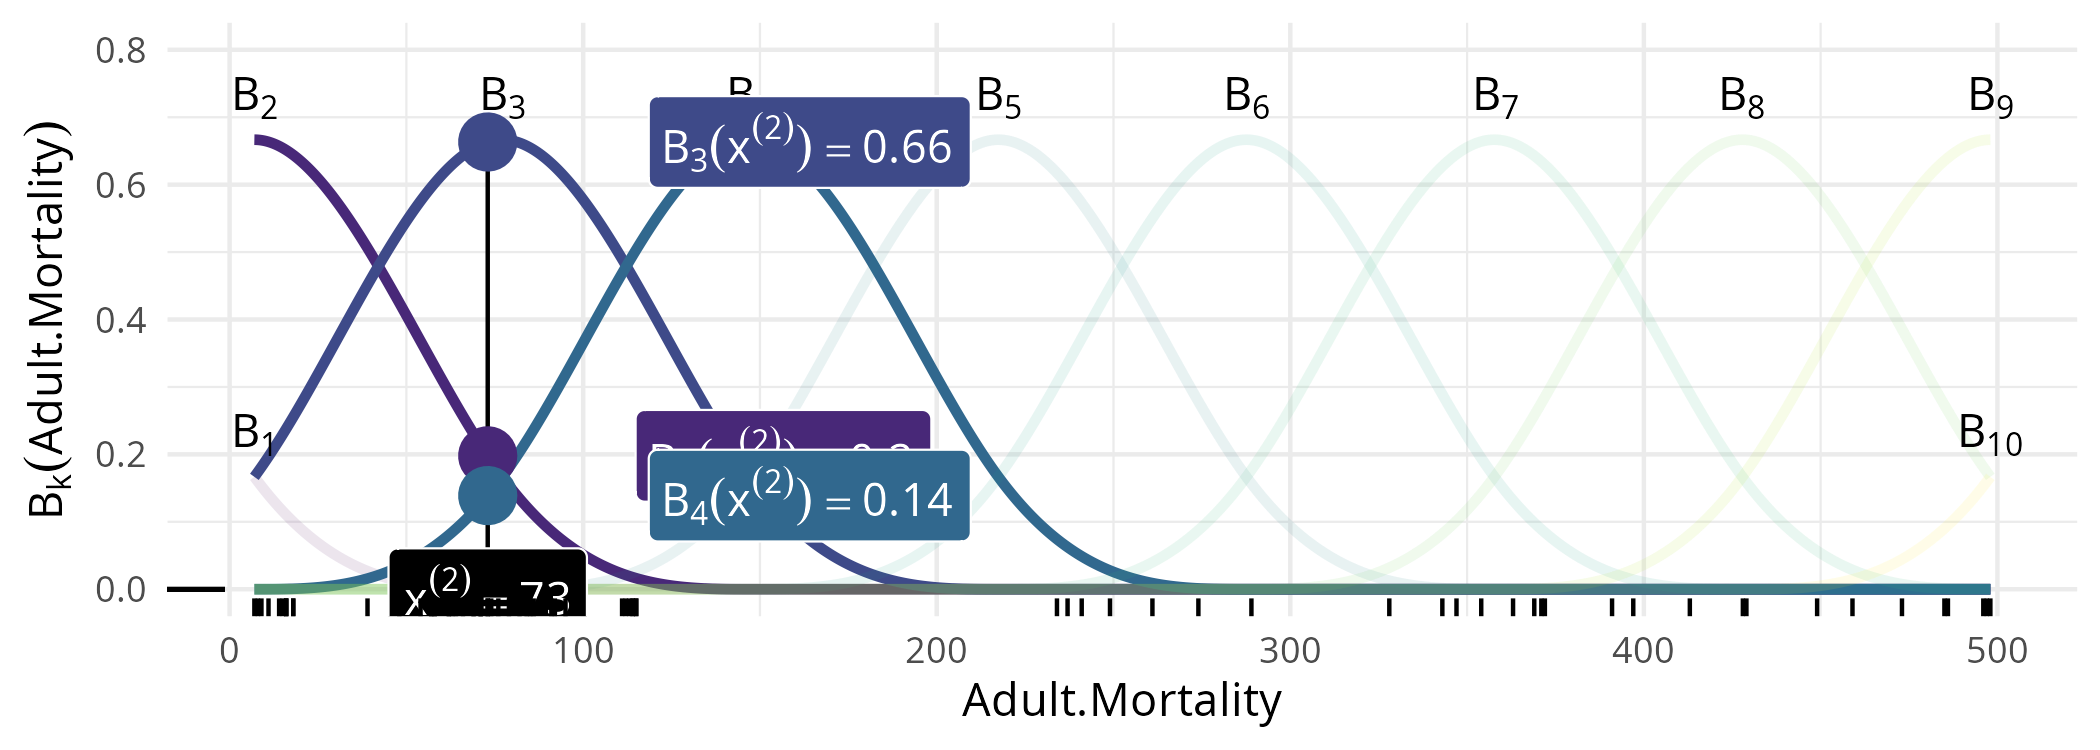
\includegraphics[width=0.7\textwidth]{figures/bs-base/fig-bs59.png}
    \end{figure}
  \end{center}
  \[
\design_k = \tiny\begin{blockarray}{cccccccccc}
\color[HTML]{440154}B_{1} & \color[HTML]{482878}B_{2} & \color[HTML]{3E4A89}B_{3} & \color[HTML]{31688E}B_{4} & \color[HTML]{26828E}B_{5} & \color[HTML]{1F9E89}B_{6} & \color[HTML]{35B779}B_{7} & \color[HTML]{6DCD59}B_{8} & \color[HTML]{B4DE2C}B_{9} & \color[HTML]{FDE725}B_{10} \\
\begin{block}{(cccccccccc)}
\phantom{x}\\
\color{lightgray}0.00 & \color{lightgray}0.00 & \color{lightgray}0.00 & \color{gray}0.07 & \color{gray}0.62 & \color{gray}0.31 & \color{lightgray}0.00 & \color{lightgray}0.00 & \color{lightgray}0.00 & \color{lightgray}0.00\color{black}\\
  \color{lightgray}0.00 & \color[HTML]{482878}0.20 & \color[HTML]{3E4A89}0.66 & \color[HTML]{31688E}0.14 & \color{lightgray}0.00 & \color{lightgray}0.00 & \color{lightgray}0.00 & \color{lightgray}0.00 & \color{lightgray}0.00 & \color{lightgray}0.00\color{black}\\
\color{white}0.00 & \color{white}0.00 & \color{white}0.00 & \color{white}0.00 & \color{white}0.00 & \color{white}0.00 & \color{white}0.00 & \color{white}0.17 & \color{white}0.67 & \color{white}0.17\color{black}\\
  \color{white}\vdots & \color{white}\vdots & \color{white}\vdots & \color{white}\vdots & \color{white}\vdots & \color{white}\vdots & \color{white}\vdots & \color{white}\vdots & \color{white}\vdots & \color{white}\vdots\\
  \color{white}0.00 & \color{white}0.02 & \color{white}0.48 & \color{white}0.48 & \color{white}0.02 & \color{white}0.00 & \color{white}0.00 & \color{white}0.00 & \color{white}0.00 & \color{white}0.00\color{black}\\
  \color{white}0.00 & \color{white}0.00 & \color{white}0.00 & \color{white}0.01 & \color{white}0.40 & \color{white}0.55 & \color{white}0.04 & \color{white}0.00 & \color{white}0.00 & \color{white}0.00\color{black}\\
  \color{white}0.00 & \color{white}0.00 & \color{white}0.00 & \color{white}0.00 & \color{white}0.00 & \color{white}0.29 & \color{white}0.63 & \color{white}0.08 & \color{white}0.00 & \color{white}0.00\color{black}\\
\phantom{x}\\
\end{block}
\end{blockarray}
\]
\normalsize

  \addtocounter{framenumber}{-1}
\end{frame}


\begin{frame}{B/P-spline base learner}
  \vspace{-0.3cm}\[g_k(x) = (B_{k,1}(x), \dots, B_{k,d_k}(x))^\tran\] B-spline basis $B$ of a pre-defined degree~\citep{eilers1996flexible}.
  \begin{center}
    \begin{figure}
      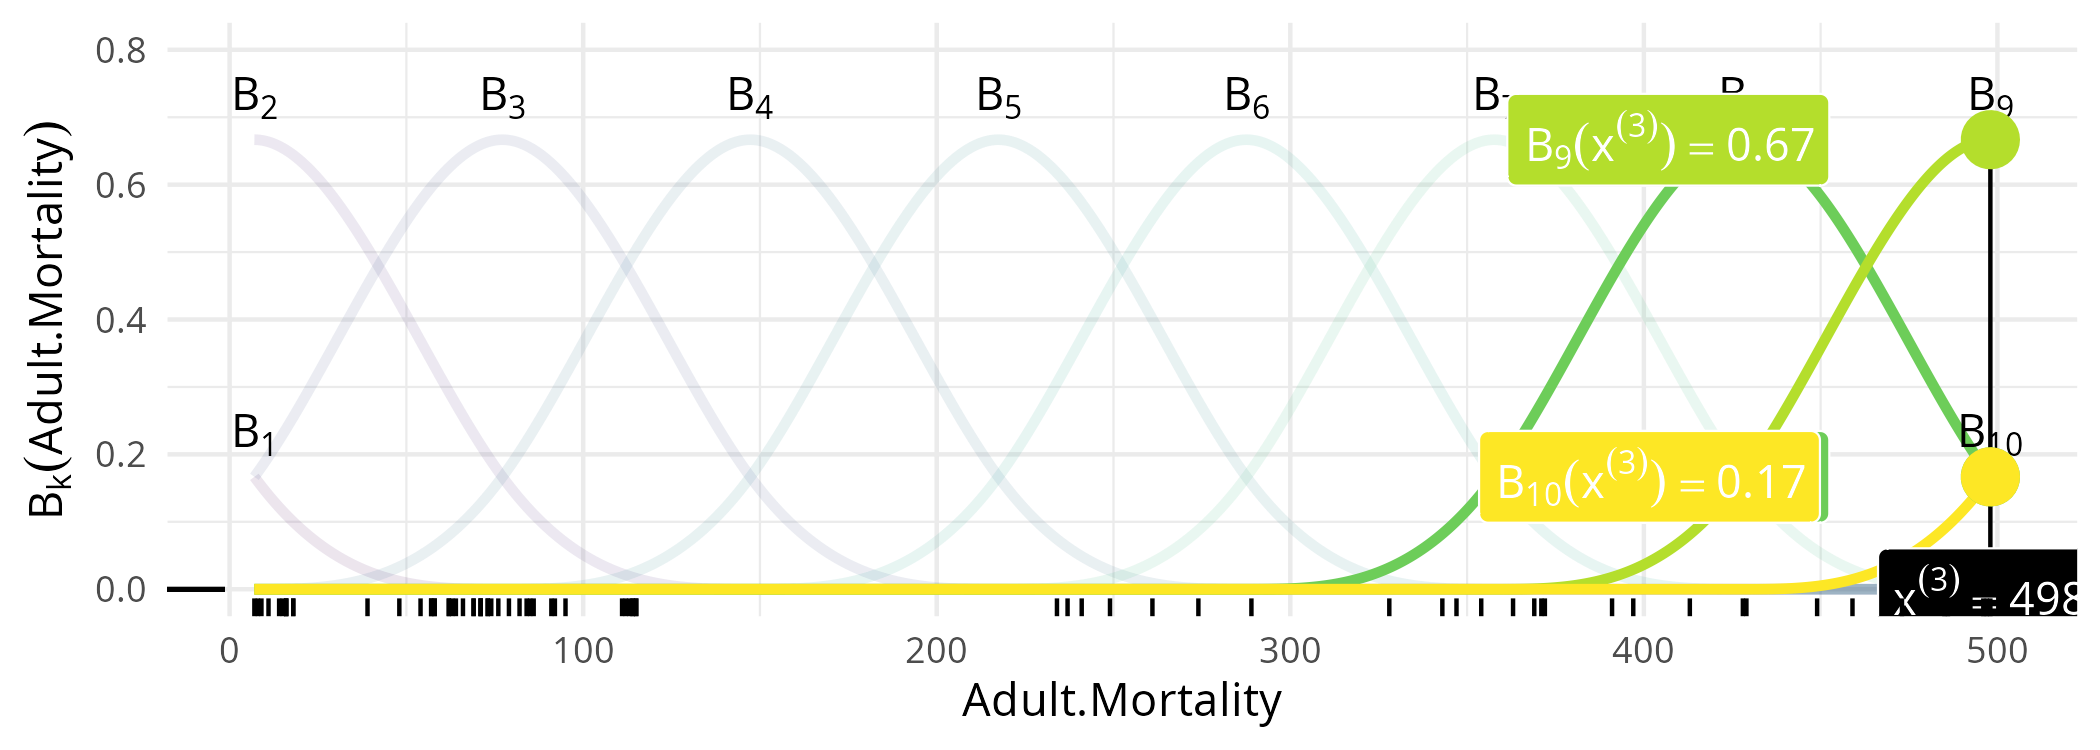
\includegraphics[width=0.7\textwidth]{figures/bs-base/fig-bs40.png}
    \end{figure}
  \end{center}
  \scriptsize
$$
\design_k = \begin{blockarray}{cccccccccc}
\color[HTML]{440154}B_{1} & \color[HTML]{482878}B_{2} & \color[HTML]{3E4A89}B_{3} & \color[HTML]{31688E}B_{4} & \color[HTML]{26828E}B_{5} & \color[HTML]{1F9E89}B_{6} & \color[HTML]{35B779}B_{7} & \color[HTML]{6DCD59}B_{8} & \color[HTML]{B4DE2C}B_{9} & \color[HTML]{FDE725}B_{10} \\
\begin{block}{(cccccccccc)}
\color{lightgray}0.00 & \color{lightgray}0.00 & \color{lightgray}0.00 & \color{gray}0.07 & \color{gray}0.62 & \color{gray}0.31 & \color{lightgray}0.00 & \color{lightgray}0.00 & \color{lightgray}0.00 & \color{lightgray}0.00\color{black}\\
  \color{lightgray}0.00 & \color{gray}0.20 & \color{gray}0.66 & \color{gray}0.14 & \color{lightgray}0.00 & \color{lightgray}0.00 & \color{lightgray}0.00 & \color{lightgray}0.00 & \color{lightgray}0.00 & \color{lightgray}0.00\color{black}\\
  \color{lightgray}0.00 & \color{lightgray}0.00 & \color{lightgray}0.00 & \color{lightgray}0.00 & \color{lightgray}0.00 & \color{lightgray}0.00 & \color{lightgray}0.00 & \color[HTML]{6DCD59}0.17 & \color[HTML]{B4DE2C}0.67 & \color[HTML]{FDE725}0.17\color{black}\\
  \color{white}\vdots & \color{white}\vdots & \color{white}\vdots & \color{white}\vdots & \color{white}\vdots & \color{white}\vdots & \color{white}\vdots & \color{white}\vdots & \color{white}\vdots & \color{white}\vdots\\
  
\end{block}
\color{white}0.00 & \color{white}0.02 & \color{white}0.48 & \color{white}0.48 & \color{white}0.02 & \color{white}0.00 & \color{white}0.00 & \color{white}0.00 & \color{white}0.00 & \color{white}0.00\color{black}\\
  \color{white}0.00 & \color{white}0.00 & \color{white}0.00 & \color{white}0.01 & \color{white}0.40 & \color{white}0.55 & \color{white}0.04 & \color{white}0.00 & \color{white}0.00 & \color{white}0.00\color{black}\\
  \color{white}0.00 & \color{white}0.00 & \color{white}0.00 & \color{white}0.00 & \color{white}0.00 & \color{white}0.29 & \color{white}0.63 & \color{white}0.08 & \color{white}0.00 & \color{white}0.00\color{black}
\end{blockarray}
$$
\normalsize

  \addtocounter{framenumber}{-1}
\end{frame}


\begin{frame}{B/P-spline base learner}
  \vspace{-0.3cm}\[g_k(x) = (B_{k,1}(x), \dots, B_{k,d_k}(x))^\tran\] B-spline basis $B$ of a pre-defined degree~\citep{eilers1996flexible}.
  \begin{center}
    \begin{figure}
      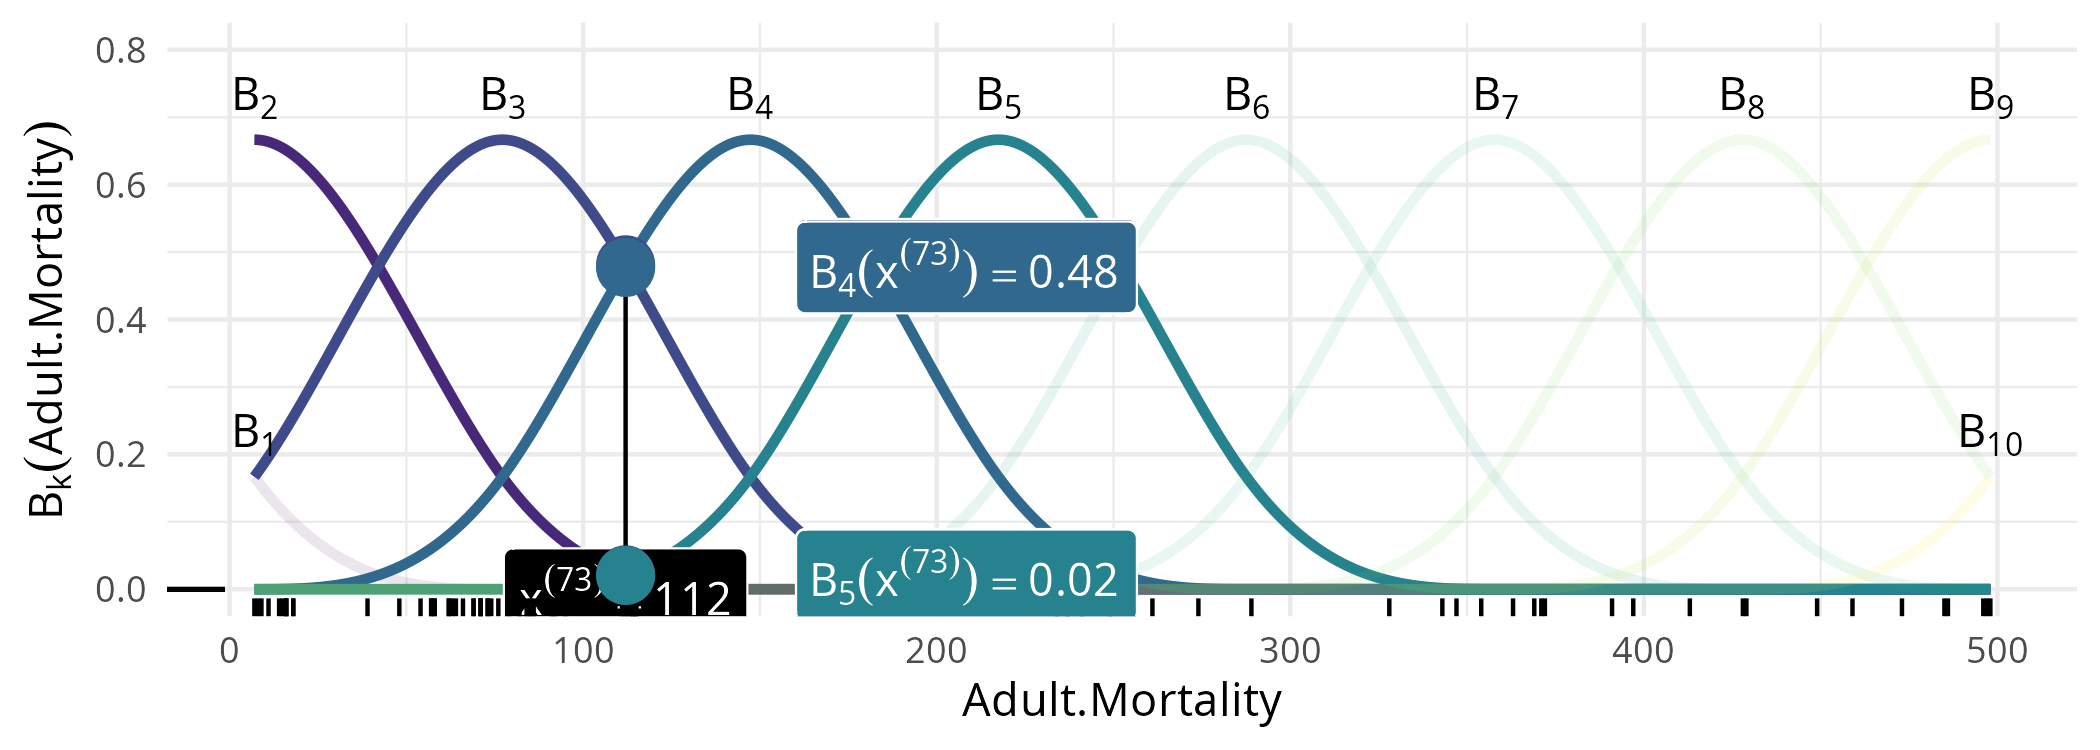
\includegraphics[width=0.7\textwidth]{figures/bs-base/fig-bs70.png}
    \end{figure}
  \end{center}
  \[
\design_k = \tiny\begin{blockarray}{cccccccccc}
\color[HTML]{440154}B_{1} & \color[HTML]{482878}B_{2} & \color[HTML]{3E4A89}B_{3} & \color[HTML]{31688E}B_{4} & \color[HTML]{26828E}B_{5} & \color[HTML]{1F9E89}B_{6} & \color[HTML]{35B779}B_{7} & \color[HTML]{6DCD59}B_{8} & \color[HTML]{B4DE2C}B_{9} & \color[HTML]{FDE725}B_{10} \\
\begin{block}{(cccccccccc)}
\phantom{x}\\
\color{lightgray}0.00 & \color{lightgray}0.00 & \color{lightgray}0.00 & \color{gray}0.07 & \color{gray}0.62 & \color{gray}0.31 & \color{lightgray}0.00 & \color{lightgray}0.00 & \color{lightgray}0.00 & \color{lightgray}0.00\color{black}\\
  \color{lightgray}0.00 & \color{gray}0.20 & \color{gray}0.66 & \color{gray}0.14 & \color{lightgray}0.00 & \color{lightgray}0.00 & \color{lightgray}0.00 & \color{lightgray}0.00 & \color{lightgray}0.00 & \color{lightgray}0.00\color{black}\\
  \color{lightgray}0.00 & \color{lightgray}0.00 & \color{lightgray}0.00 & \color{lightgray}0.00 & \color{lightgray}0.00 & \color{lightgray}0.00 & \color{lightgray}0.00 & \color{gray}0.17 & \color{gray}0.67 & \color{gray}0.17\color{black}\\
  \color{black}\vdots & \color{black}\vdots & \color{black}\vdots & \color{black}\vdots & \color{black}\vdots & \color{black}\vdots & \color{black}\vdots & \color{black}\vdots & \color{black}\vdots & \color{black}\vdots\\
  \color{lightgray}0.00 & \color[HTML]{482878}0.02 & \color[HTML]{3E4A89}0.48 & \color[HTML]{31688E}0.48 & \color[HTML]{26828E}0.02 & \color{lightgray}0.00 & \color{lightgray}0.00 & \color{lightgray}0.00 & \color{lightgray}0.00 & \color{lightgray}0.00\color{black}\\
\color{white}0.00 & \color{white}0.00 & \color{white}0.00 & \color{white}0.01 & \color{white}0.40 & \color{white}0.55 & \color{white}0.04 & \color{white}0.00 & \color{white}0.00 & \color{white}0.00\color{black}\\
  \color{white}0.00 & \color{white}0.00 & \color{white}0.00 & \color{white}0.00 & \color{white}0.00 & \color{white}0.29 & \color{white}0.63 & \color{white}0.08 & \color{white}0.00 & \color{white}0.00\color{black}\\
\phantom{x}\\
\end{block}
\end{blockarray}
\]
\normalsize

  \addtocounter{framenumber}{-1}
\end{frame}


\begin{frame}{B/P-spline base learner}
  \vspace{-0.3cm}\[g_k(x) = (B_{k,1}(x), \dots, B_{k,d_k}(x))^\tran\] B-spline basis $B$ of a pre-defined degree~\citep{eilers1996flexible}.
  \begin{center}
    \begin{figure}
      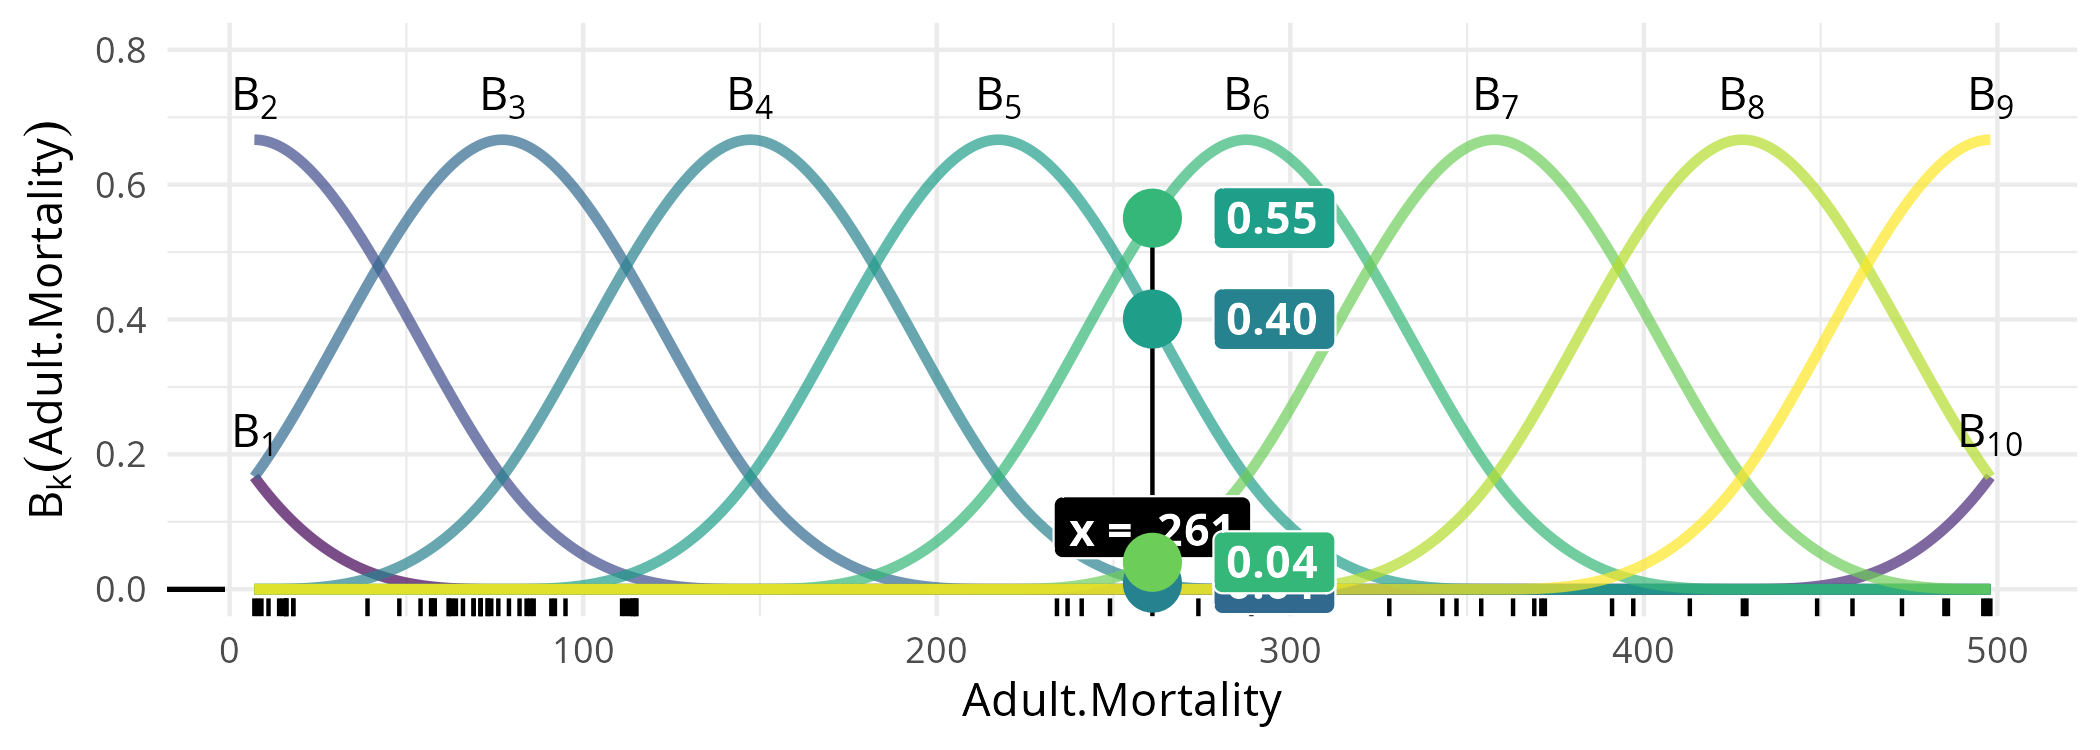
\includegraphics[width=0.7\textwidth]{figures/bs-base/fig-bs5.png}
    \end{figure}
  \end{center}
  \[
\design_k = \tiny\begin{blockarray}{cccccccccc}
\color[HTML]{440154}B_{1} & \color[HTML]{482878}B_{2} & \color[HTML]{3E4A89}B_{3} & \color[HTML]{31688E}B_{4} & \color[HTML]{26828E}B_{5} & \color[HTML]{1F9E89}B_{6} & \color[HTML]{35B779}B_{7} & \color[HTML]{6DCD59}B_{8} & \color[HTML]{B4DE2C}B_{9} & \color[HTML]{FDE725}B_{10} \\
\begin{block}{(cccccccccc)}
\phantom{x}\\
\color{lightgray}0.00 & \color{lightgray}0.00 & \color{lightgray}0.00 & \color{gray}0.07 & \color{gray}0.62 & \color{gray}0.31 & \color{lightgray}0.00 & \color{lightgray}0.00 & \color{lightgray}0.00 & \color{lightgray}0.00\color{black}\\
  \color{lightgray}0.00 & \color{gray}0.20 & \color{gray}0.66 & \color{gray}0.14 & \color{lightgray}0.00 & \color{lightgray}0.00 & \color{lightgray}0.00 & \color{lightgray}0.00 & \color{lightgray}0.00 & \color{lightgray}0.00\color{black}\\
  \color{lightgray}0.00 & \color{lightgray}0.00 & \color{lightgray}0.00 & \color{lightgray}0.00 & \color{lightgray}0.00 & \color{lightgray}0.00 & \color{lightgray}0.00 & \color{gray}0.17 & \color{gray}0.67 & \color{gray}0.17\color{black}\\
  \color{black}\vdots & \color{black}\vdots & \color{black}\vdots & \color{black}\vdots & \color{black}\vdots & \color{black}\vdots & \color{black}\vdots & \color{black}\vdots & \color{black}\vdots & \color{black}\vdots\\
  \color{lightgray}0.00 & \color{gray}0.02 & \color{gray}0.48 & \color{gray}0.48 & \color{gray}0.02 & \color{lightgray}0.00 & \color{lightgray}0.00 & \color{lightgray}0.00 & \color{lightgray}0.00 & \color{lightgray}0.00\color{black}\\
  \color{lightgray}0.00 & \color{lightgray}0.00 & \color{lightgray}0.00 & \color[HTML]{31688E}0.01 & \color[HTML]{26828E}0.40 & \color[HTML]{1F9E89}0.55 & \color[HTML]{35B779}0.04 & \color{lightgray}0.00 & \color{lightgray}0.00 & \color{lightgray}0.00\color{black}\\
\color{white}0.00 & \color{white}0.00 & \color{white}0.00 & \color{white}0.00 & \color{white}0.00 & \color{white}0.29 & \color{white}0.63 & \color{white}0.08 & \color{white}0.00 & \color{white}0.00\color{black}\\
\phantom{x}\\
\end{block}
\end{blockarray}
\]
\normalsize

  \addtocounter{framenumber}{-1}
\end{frame}


\begin{frame}{B/P-spline base learner}
  \vspace{-0.3cm}\[g_k(x) = (B_{k,1}(x), \dots, B_{k,d_k}(x))^\tran\] B-spline basis $B$ of a pre-defined degree~\citep{eilers1996flexible}.
  \begin{center}
    \begin{figure}
      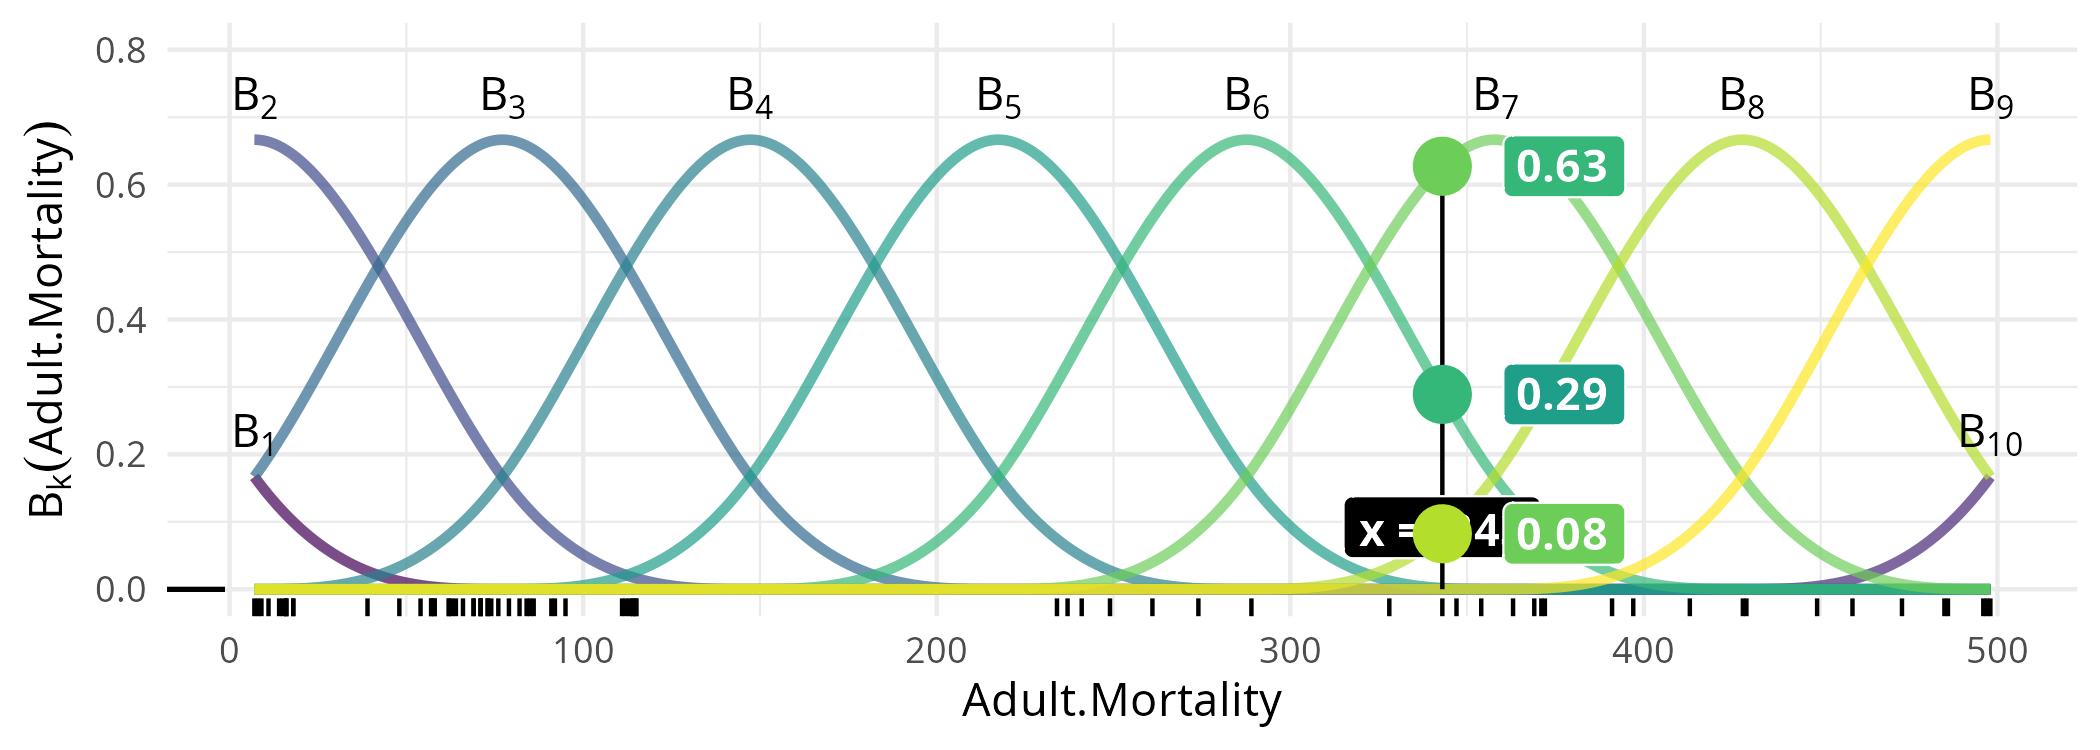
\includegraphics[width=0.7\textwidth]{figures/bs-base/fig-bs10.png}
    \end{figure}
  \end{center}
  \[
\design_k = \tiny\begin{blockarray}{cccccccccc}
\color[HTML]{440154}B_{1} & \color[HTML]{482878}B_{2} & \color[HTML]{3E4A89}B_{3} & \color[HTML]{31688E}B_{4} & \color[HTML]{26828E}B_{5} & \color[HTML]{1F9E89}B_{6} & \color[HTML]{35B779}B_{7} & \color[HTML]{6DCD59}B_{8} & \color[HTML]{B4DE2C}B_{9} & \color[HTML]{FDE725}B_{10} \\
\begin{block}{(cccccccccc)}
\phantom{x}\\
\color{lightgray}0.00 & \color{lightgray}0.00 & \color{lightgray}0.00 & \color{gray}0.07 & \color{gray}0.62 & \color{gray}0.31 & \color{lightgray}0.00 & \color{lightgray}0.00 & \color{lightgray}0.00 & \color{lightgray}0.00\color{black}\\
  \color{lightgray}0.00 & \color{gray}0.20 & \color{gray}0.66 & \color{gray}0.14 & \color{lightgray}0.00 & \color{lightgray}0.00 & \color{lightgray}0.00 & \color{lightgray}0.00 & \color{lightgray}0.00 & \color{lightgray}0.00\color{black}\\
  \color{lightgray}0.00 & \color{lightgray}0.00 & \color{lightgray}0.00 & \color{lightgray}0.00 & \color{lightgray}0.00 & \color{lightgray}0.00 & \color{lightgray}0.00 & \color{gray}0.17 & \color{gray}0.67 & \color{gray}0.17\color{black}\\
  \color{black}\vdots & \color{black}\vdots & \color{black}\vdots & \color{black}\vdots & \color{black}\vdots & \color{black}\vdots & \color{black}\vdots & \color{black}\vdots & \color{black}\vdots & \color{black}\vdots\\
  \color{lightgray}0.00 & \color{gray}0.02 & \color{gray}0.48 & \color{gray}0.48 & \color{gray}0.02 & \color{lightgray}0.00 & \color{lightgray}0.00 & \color{lightgray}0.00 & \color{lightgray}0.00 & \color{lightgray}0.00\color{black}\\
  \color{lightgray}0.00 & \color{lightgray}0.00 & \color{lightgray}0.00 & \color{gray}0.01 & \color{gray}0.40 & \color{gray}0.55 & \color{gray}0.04 & \color{lightgray}0.00 & \color{lightgray}0.00 & \color{lightgray}0.00\color{black}\\
  \color{lightgray}0.00 & \color{lightgray}0.00 & \color{lightgray}0.00 & \color{lightgray}0.00 & \color{lightgray}0.00 & \color[HTML]{1F9E89}0.29 & \color[HTML]{35B779}0.63 & \color[HTML]{6DCD59}0.08 & \color{lightgray}0.00 & \color{lightgray}0.00\color{black}\\
\phantom{x}\\
\end{block}
\end{blockarray}
\]
\normalsize

  \addtocounter{framenumber}{-1}
\end{frame}

